\textbf{مورد استفاده:}
داشبورد مدیریت
\\
\textbf{شرح مختصر :UC}
در این قسمت داشبورد مدیریت را در اختیار کاربر قرار می‌دهد.
\\
\textbf{پيش شرط:}
ورود کاربر با سطح دسترسی مدیر.
\\
\textbf{سناريو اصلی:}
\begin{enumerate}
	\item
	شروع
	\item
	مدیر به بخش‌های مختلف مانند ایجاد و حذف کاربر، تعیین سطوح دسترسی کاربران و .. دسترسی پیدا می‌کند.
	\item
	پایان
\end{enumerate}

\noindent
\textbf{پس شرط:}
ندارد.
\\
\textbf{سناريوهای فرعی:}
ندارد.
\\
\textbf{پس شرط:}
ندارد.


\begin{figure}[H]
	\centering
	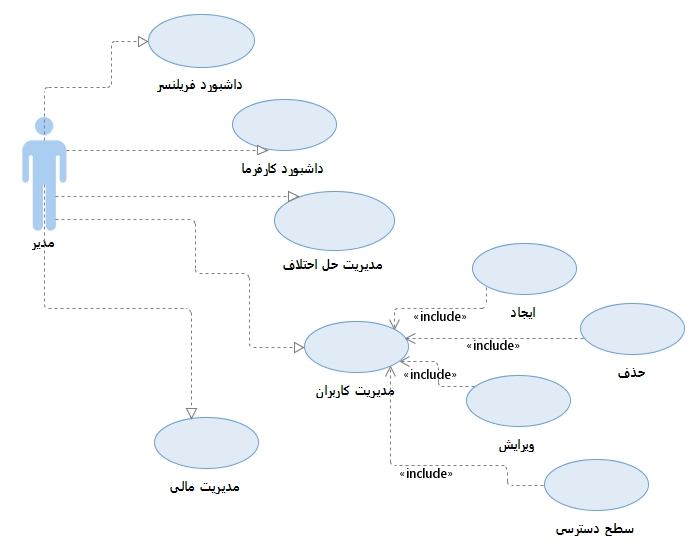
\includegraphics[width=0.7\textwidth]{Diagram/1.UseCase/داشبورد-مدیریت.png}
	\caption{دیاگرام UC داشبورد مدیریت}
	\label{fig:uc:داشبورد-مدیریت}
\end{figure}